\documentclass{article}
%\usepackage{geometry}
%\geometry{top = 1in, bottom = 1in, left = 1in, right = 1in}
\usepackage[top = 0.7in, bottom = 0.7in, left = 0.7in, right = 0.7in]{geometry}
\usepackage{amsmath,amssymb,amsthm,mathrsfs}
\usepackage{graphicx}
\usepackage{bm}
\usepackage{float}
\usepackage[font=footnotesize,labelfont=bf]{caption}
\usepackage{movie15}
\usepackage{hyperref}

\usepackage{fancyhdr}
\pagestyle{fancy}
\rhead{\footnotesize {09/17/2012 ; MESA version 4493} }
\chead{\footnotesize {Authors: Jared Brooks, Lars Bildsten, Bill Paxton} }
\lhead{\footnotesize {mesa/star/test\_suite/massive\_rotating} }

\begin{document}
	
	\begin{center}
	  \begin{Large}
	    \textbf{MASSIVE ROTATING}\\
	  \end{Large}
	\end{center}

        This test is to show a 15 $M_\odot$ rapidly rotating star.  It starts with pre-main sequence model and evolves it until the mass fraction for center neon reaches 0.25 (\texttt{xa\_central\_upper\_limit\_species(1) = 'ne20' ; xa\_central\_upper\_limit(1) = 0.25}).\\

        There are two inlists for this test.  The first inlist creates the 15 $M_\odot$ pre-main sequence model and evolves it until the nuclear burning luminosity reaches surface luminosity (\texttt{Lnuc\_div\_L\_upper\_limit = 1}).  The second inlist sets a uniform rotational frequency to give surface omega = 0.5$\times$critical omega for the first 10 steps with the following controls:
        \begin{itemize}
        \item \texttt{change\_rotation\_flag = .true.}
        \item \texttt{new\_rotation\_flag = .true.}
        \item \texttt{set\_initial\_omega\_div\_omega\_crit = .true.}
        \item \texttt{new\_omega\_div\_omega\_crit = 0.5}
        \item \texttt{set\_omega\_div\_omega\_crit\_step\_limit = 10}
        \end{itemize}

        The HR-diagram below shows the evolution from the second inlist (figure \ref{fig:1}), with some important features marked by the colored dots.  The red dot marks the end of core hydrogen burning.  The blue dot marks the start of core helium burning.  The green dot marks the end of core helium burning.  The orange dots mark the two points when the surface rotation frequency reaches the critical rotation frequency and significant mass loss occurs as a result.

        \begin{figure}[H]
          \centering
          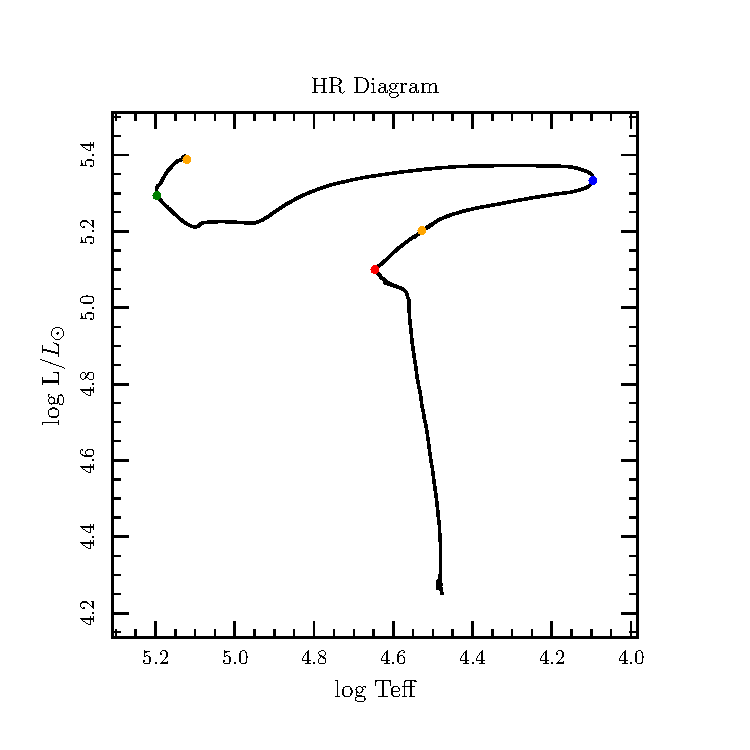
\includegraphics[width = 5in]{/Users/jaredbrooks/massive_rotating/plots_out/HR_Diagram.pdf}
          \caption{Red: end of core H burning, Blue: start of core He burning, Green: end of core He burning, Orange: critical rotation rates}
          \label{fig:1}
        \end{figure}

        \pagebreak

        The star keeps its relative surface rotation frequency until the first orange dot, starting just after 19.7 Myr.  The plot to the left shows the evolution of the relative surface rotation frequency (figure \ref{fig:2}).  The plot to the right shows the log of the factor of increased mass loss rate due to rotation (e.g. factor of 1 means no additional mass loss from rotation, factor of 2 means rotation has doubled the mass loss rate).  During the two peaks shown, rotation increased mass loss by a factor of $10^6$ (figure \ref{fig:3}).

        \begin{figure}[H]
          \begin{minipage}[b]{0.5\linewidth}
	    \centering
	    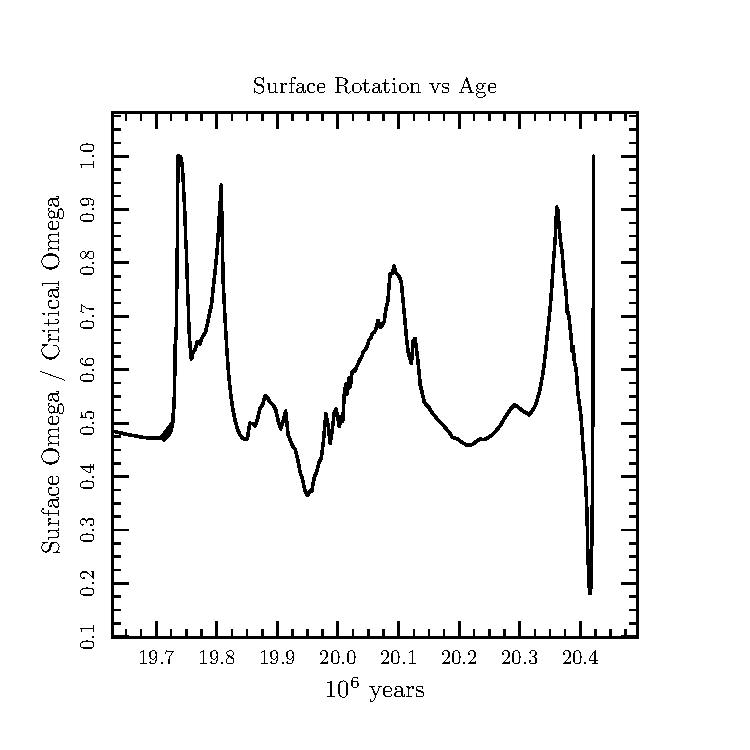
\includegraphics[width = 3.7in]{/Users/jaredbrooks/massive_rotating/plots_out/Surface_Rotation_vs_Age.pdf}
	    \caption{Surface omega/critical omega}
	    \label{fig:2}
          \end{minipage}
          \hspace{0cm}
          \begin{minipage}[b]{0.5\linewidth}
            \centering
            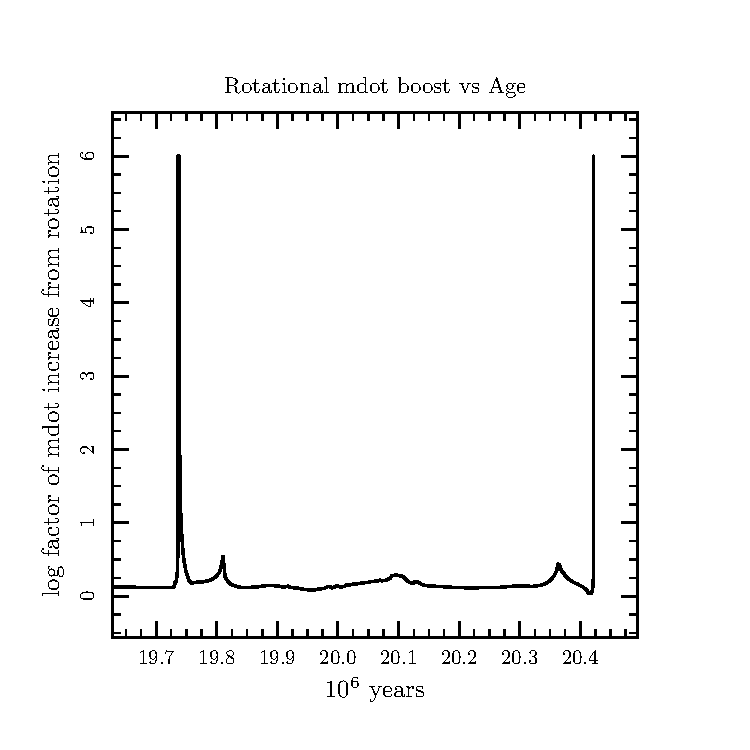
\includegraphics[width = 3.7in]{/Users/jaredbrooks/massive_rotating/plots_out/Rotational_Mdot_Boost_vs_Age.pdf}
            \caption{log of factor of increase in mass loss rate due to rotation}
            \label{fig:3}
          \end{minipage}
	\end{figure}

        To the left is a plot of the mass and total angular momentum for the last 6 Myr of the run (figure \ref{fig:4}).  To the right is a plot of the evolution of the center temperature and density (figure \ref{fig:5}).

        \begin{figure}[H]
            \begin{minipage}[b]{0.5\linewidth}
            \centering
            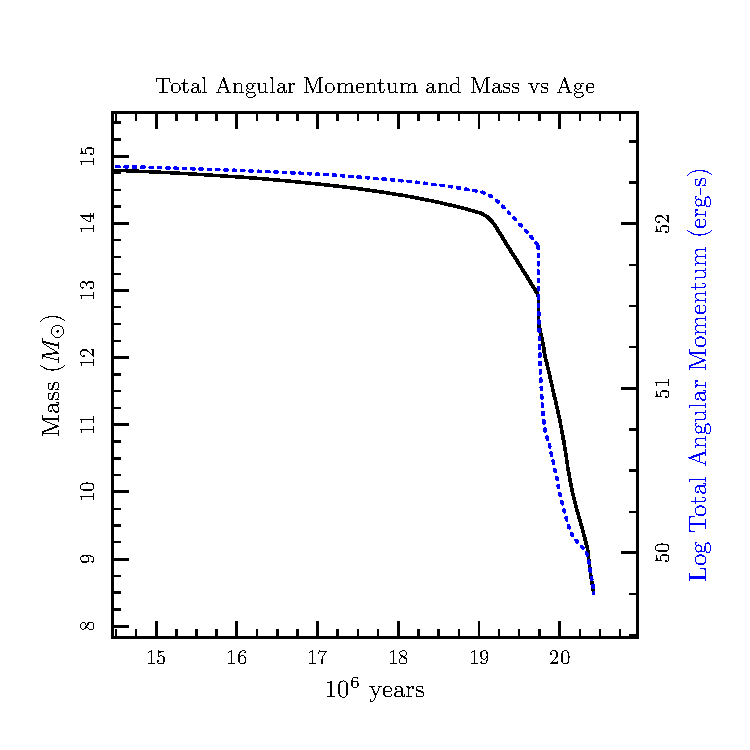
\includegraphics[width = 3.7in]{/Users/jaredbrooks/massive_rotating/plots_out/Total_Angular_Momentum_vs_Age.pdf}
            \caption{}
            \label{fig:4}
          \end{minipage}
          \hspace{0cm}
          \begin{minipage}[b]{0.5\linewidth}
            \centering
            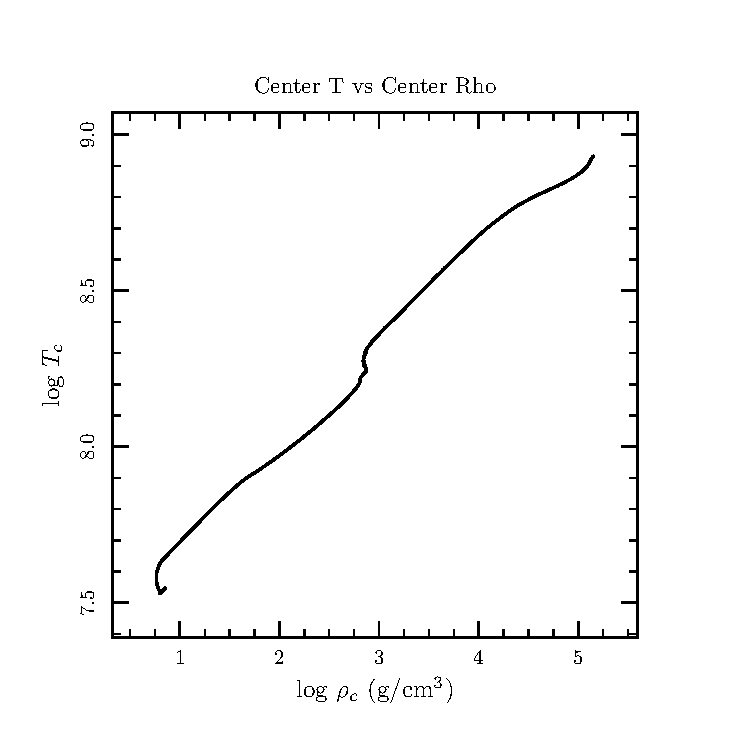
\includegraphics[width = 3.7in]{/Users/jaredbrooks/massive_rotating/plots_out/Tc_vs_Rhoc.pdf}
            \caption{}
            \label{fig:5}
          \end{minipage}
        \end{figure}

        \pagebreak

        All of the plots on this page are profile from the first orange dot on the HR-diagram (figure \ref{fig:1}).  The following two profiles show the magnetic fields generated by the Taylor-Spruit dynamo in the poloidal (radial) and toroidal (azimuthal) components.  The profile to the left (figure \ref{fig:6}) shows that these magnetic fields are only being generated in the radiative region between convection zones.  The profile to the right (figure \ref{fig:7}) shows how magnetic field generation is affected by rotation rate.

        \begin{figure}[H]
          \begin{minipage}[b]{0.5\linewidth}
            \centering
            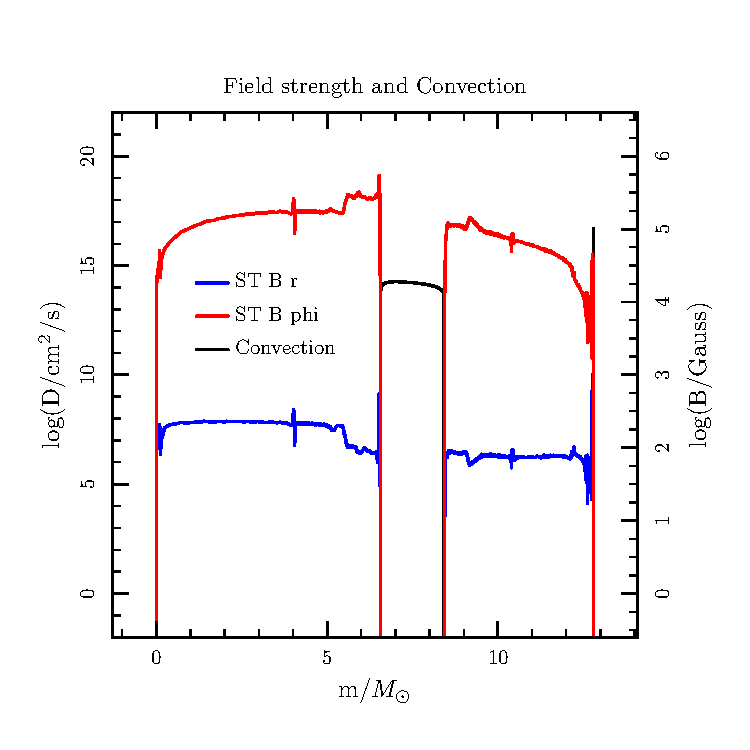
\includegraphics[width = 3.6in]{/Users/jaredbrooks/massive_rotating/plots_out/B_and_Conv_vs_mass_23.pdf}
            \caption{Magnetic field generation and Convection at first orange dot}
            \label{fig:6}
          \end{minipage}
          \hspace{0cm}
          \begin{minipage}[b]{0.5\linewidth}
            \centering
            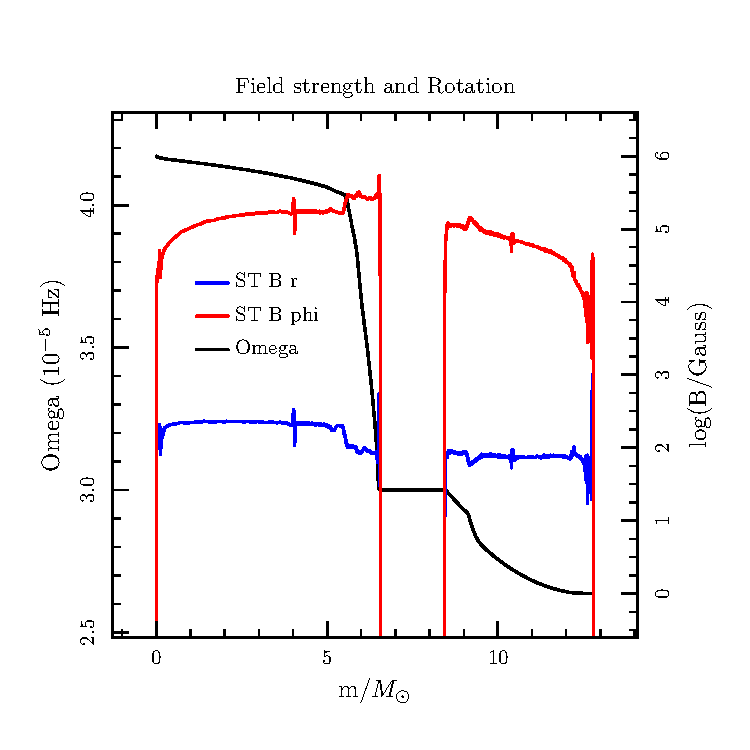
\includegraphics[width = 3.6in]{/Users/jaredbrooks/massive_rotating/plots_out/B_and_omega_vs_mass_23.pdf}
            \caption{Magnetic field generation and Rotation frequency at first orange dot}
            \label{fig:7}
          \end{minipage}
        \end{figure}

        The profile to the left shows a number of diffusion coefficients (figure \ref{fig:8}).  To the right is a burning rate profile (figure \ref{fig:9}).

        \begin{figure}[H]
          \begin{minipage}[b]{0.5\linewidth}
            \centering
            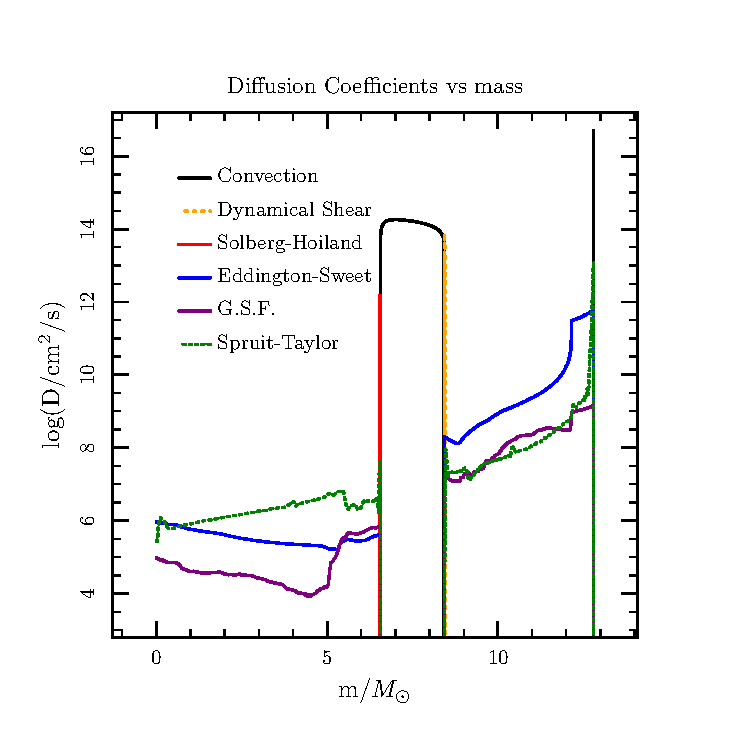
\includegraphics[width = 3.6in]{/Users/jaredbrooks/massive_rotating/plots_out/Diffusion_Coefficients_vs_mass_23.pdf}
            \caption{Diffusion coefficients at first orange dot}
            \label{fig:8}
          \end{minipage}
          \hspace{0cm}
          \begin{minipage}[b]{0.5\linewidth}
            \centering
            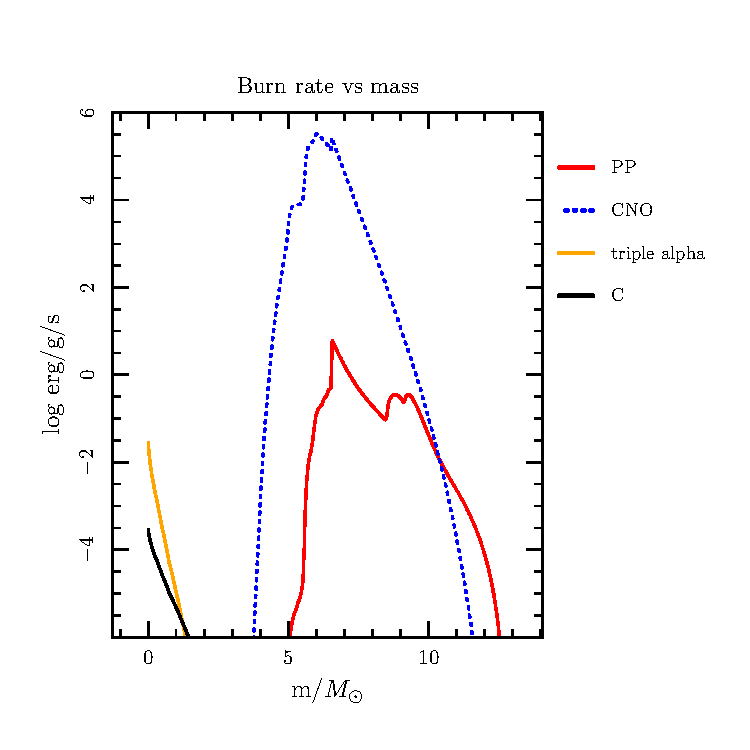
\includegraphics[width = 3.6in]{/Users/jaredbrooks/massive_rotating/plots_out/Burnrate_vs_mass_23.pdf}
            \caption{Burning rate profile at first orange dot}
            \label{fig:9}
          \end{minipage}
        \end{figure}

        \pagebreak

        All of the plots on this page are profile from the second orange dot on the HR-diagram (figure \ref{fig:1}).  The following two profiles show the magnetic fields generated by the Taylor-Spruit dynamo in the poloidal (radial) and toroidal (azimuthal) components.  The profile to the left (figure \ref{fig:10}) shows that these magnetic fields are only being generated in the radiative region between convection zones.  The profile to the right (figure \ref{fig:11}) shows how magnetic field generation is affected by rotation rate.

        \begin{figure}[H]
          \begin{minipage}[b]{0.5\linewidth}
            \centering
            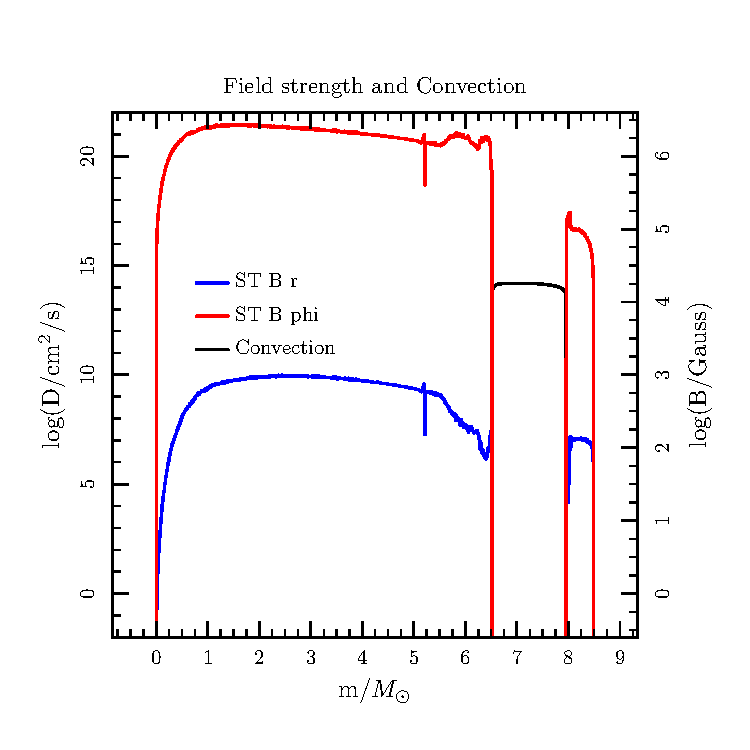
\includegraphics[width = 3.6in]{/Users/jaredbrooks/massive_rotating/plots_out/B_and_Conv_vs_mass_69.pdf}
            \caption{Magnetic field generation and Convection at second orange dot}
            \label{fig:10}
          \end{minipage}
          \hspace{0cm}
          \begin{minipage}[b]{0.5\linewidth}
            \centering
            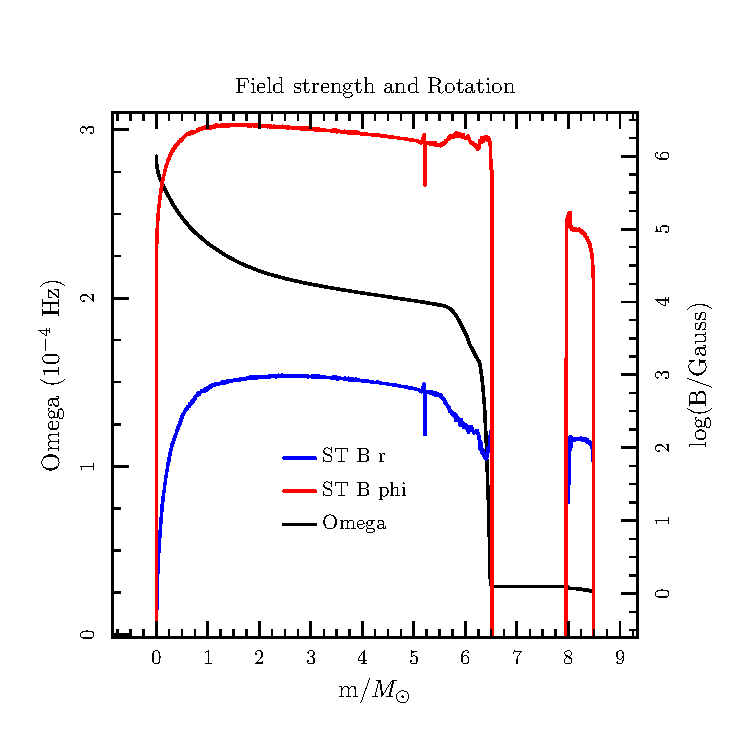
\includegraphics[width = 3.6in]{/Users/jaredbrooks/massive_rotating/plots_out/B_and_omega_vs_mass_69.pdf}
            \caption{Magnetic field generation and Rotation frequency at second orange dot}
            \label{fig:11}
          \end{minipage}
        \end{figure}
        
        The profile to the left shows a number of diffusion coefficients (figure \ref{fig:12}).  To the right is a burning rate profile (figure \ref{fig:13}).
        
        \begin{figure}[H]
          \begin{minipage}[b]{0.5\linewidth}
            \centering
            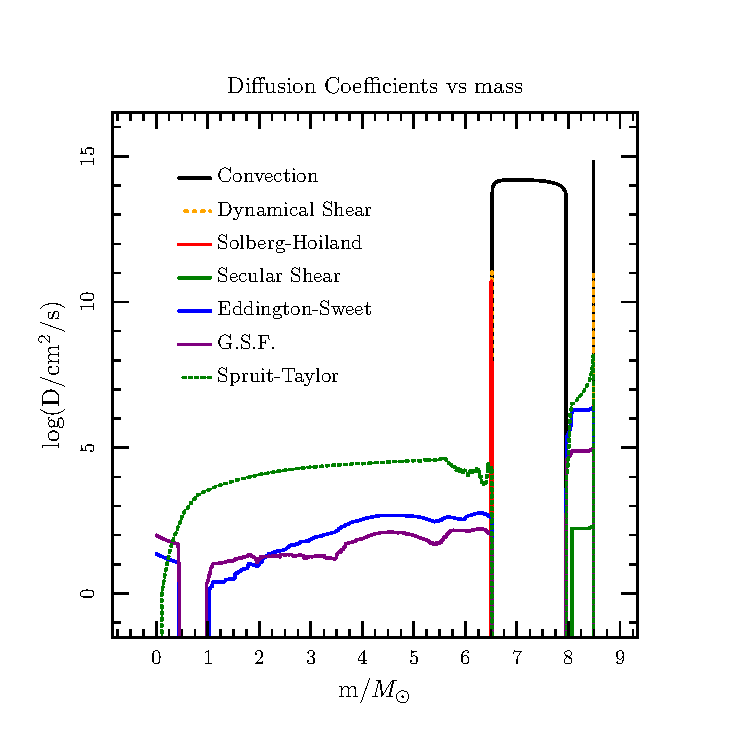
\includegraphics[width = 3.6in]{/Users/jaredbrooks/massive_rotating/plots_out/Diffusion_Coefficients_vs_mass_69.pdf}
            \caption{Diffusion coefficients at second orange dot}
            \label{fig:12}
          \end{minipage}
          \hspace{0cm}
          \begin{minipage}[b]{0.5\linewidth}
            \centering
            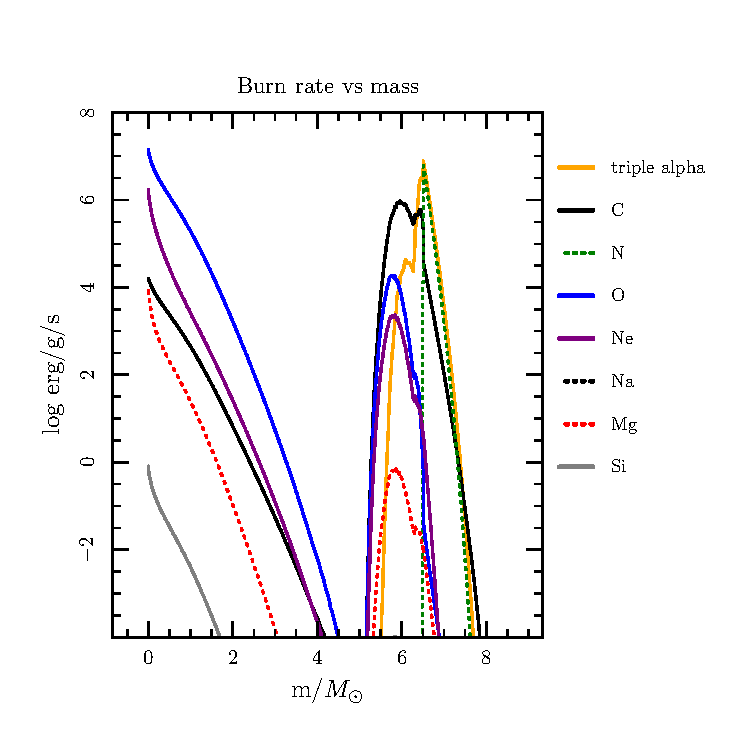
\includegraphics[width = 3.6in]{/Users/jaredbrooks/massive_rotating/plots_out/Burnrate_vs_mass_69.pdf}
            \caption{Burning rate profile at second orange dot}
            \label{fig:13}
          \end{minipage}
        \end{figure}

        \pagebreak

        Below is a profile of the abundances at the end of the run (figure \ref{fig:14}).

        \begin{figure}[H]
          \centering
          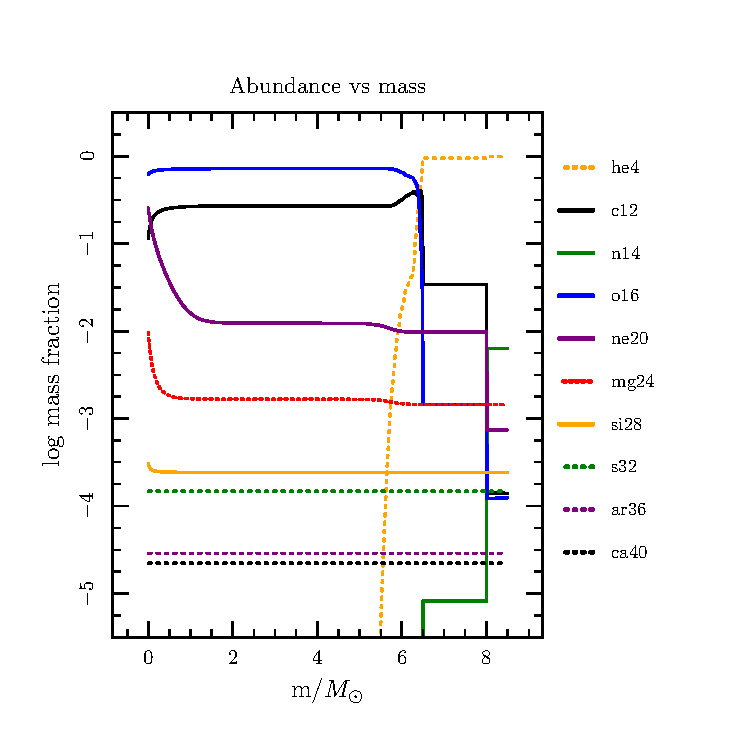
\includegraphics[width = 5in]{/Users/jaredbrooks/massive_rotating/plots_out/Abundance_vs_mass_71.pdf}
          \caption{Abundance profile from end of run}
          \label{fig:14}
        \end{figure}

        \pagebreak

        This final plot (figure \ref{fig:15}) shows a few internal \texttt{MESA} variables, such as the size of the time-step, the number of zones, and the number of retries against the model number in order to give some understanding of how hard \texttt{MESA} is working throughout the run and where some areas of problems/interest might be.

        \begin{figure}[H]
          \centering
          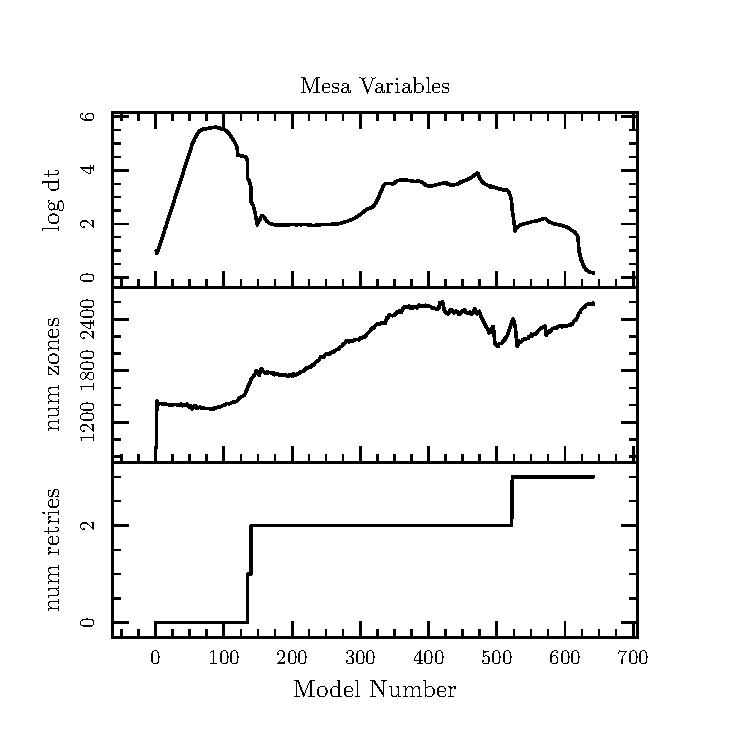
\includegraphics[width = 5in]{/Users/jaredbrooks/massive_rotating/plots_out/Mesa_Variables.pdf}
          \caption{\texttt{MESA} variables plotted against model number show how hard \texttt{MESA} is working}
          \label{fig:15}
        \end{figure}


\end{document}
